\documentclass[a4paper]{article}
\usepackage{color}
\usepackage{url}
\usepackage{fontenc} % enable Cyrillic fonts
\usepackage[utf8]{inputenc} % make weird characters work
\usepackage{graphicx} 
\usepackage[english]{babel}
% \usepackage[english,serbianc]{babel} %ukljuciti babel sa ovim opcijama, umesto gornjim, ukoliko se koristi cirilica

\usepackage[unicode]{hyperref}
\hypersetup{colorlinks,citecolor=green,filecolor=green,linkcolor=blue,urlcolor=blue}

\usepackage{listings}
% 
% %\newtheorem{primer}{Пример}[section] %ćirilični primer
\newtheorem{primer}{Primer}[section]
% 
\definecolor{mygreen}{rgb}{0,0.6,0}
\definecolor{mygray}{rgb}{0.5,0.5,0.5}
\definecolor{mymauve}{rgb}{0.58,0,0.82}
\lstset{ 
   backgroundcolor=\color{white},   % choose the background color; you must add \usepackage{color} or \usepackage{xcolor}; should come as last argument
   basicstyle=\scriptsize\ttfamily,        % the size of the fonts that are used for the code
   breakatwhitespace=false,         % sets if automatic breaks should only happen at whitespace
   breaklines=true,                 % sets automatic line breaking
   captionpos=b,                    % sets the caption-position to bottom
   commentstyle=\color{mygreen},    % comment style
   deletekeywords={...},            % if you want to delete keywords from the given language
   escapeinside={\%*}{*)},          % if you want to add LaTeX within your code
   extendedchars=true,              % lets you use non-ASCII characters; for 8-bits encodings only, does not work with UTF-8
   firstnumber=1000,                % start line enumeration with line 1000
   frame=single,	                   % adds a frame around the code
   keepspaces=true,                 % keeps spaces in text, useful for keeping indentation of code (possibly needs columns=flexible)
   keywordstyle=\color{blue},       % keyword style
   language=Python,                 % the language of the code
   morekeywords={*,...},            % if you want to add more keywords to the set
   numbers=left,                    % where to put the line-numbers; possible values are (none, left, right)
   numbersep=5pt,                   % how far the line-numbers are from the code
   numberstyle=\tiny\color{mygray}, % the style that is used for the line-numbers
   rulecolor=\color{black},         % if not set, the frame-color may be changed on line-breaks within not-black text (e.g. comments (green here))
   showspaces=false,                % show spaces everywhere adding particular underscores; it overrides 'showstringspaces'
   showstringspaces=false,          % underline spaces within strings only
   showtabs=false,                  % show tabs within strings adding particular underscores
   stepnumber=2,                    % the step between two line-numbers. If it's 1, each line will be numbered
   stringstyle=\color{mymauve},     % string literal style
   tabsize=2,	                   % sets default tabsize to 2 spaces
   title=\lstname                   % show the filename of files included with \lstinputlisting; also try caption instead of title
 }


\begin{document}
	
	\title{Komunikacija preko mreže\\ \small{Seminarski rad u okviru kursa\\Metodologija stručnog i naučnog rada\\ Matematički fakultet}}
	
	\author{Bakić Katarina, Nenad , Kovačević Matija, Kovačević Nikola\\ ina.bakic95@gmail.com, drugog, trećeg, četvrtog autora}
	
	\date{6.april 2019.}
	
	\maketitle
	\abstract{
		Mrežne komunikacije imaju poseban značaj poslednjih godina, njenim razvojem je omogućeno poslovanje među firmama, pristup određenim nedostižnim informacijama, prodaja, kupovina, komunikacija sa prijateljima putem društvenih mreža. Internet je globalna mreža koja nam daje mogućnost komunikacije i deljenja resursa na Zemlji. Ovaj vid komunikacije nam omogucava da u svakom trenutku pronađemo ono sto nam treba od podataka. Programerski poslovi su postali sve aktuelniji i plaćeniji. Koliko god prednosti da ima, toliko ima i mana. Ljudi sve više vremena provode za računarima, pametnim telefonima i sličnim uređajima. Deca nam sve manje izlaze na igrališta sa svojim vršnjacima, sada je aktuelno igranje igrica , pa se samim tim javlja velika zavisnost i zdravstveni problem sa vidom. Komunikacija se ne odvija samo putem telefona i računara, dosta je zastupljena i u auto industiriji, kao na primer da pojedini automobili  imaju mogućnost da snimaju razgovore, koji kasnije mogu da se iskoriste, ukoliko dođe do nesreće.Većina uređaja ima GPS, pa samim tim se sve više prate naša kretanja.U medicine se takođe sve više koristi internet, mnogi uređaji za lečenja se zasnivaju na njemu. Računari i računarske mreže se danas takođe mogu zloupotrebljavati na razne načine.\\
		\begin{primer}
		Upravo tako, sve se pretvara u kompjuter.Vaš telefon je kompjuter koji poziva. Vaš automobil je kompjuter sa točkovima i motorom.Vaša pećnica je kompjuter, koji pravi lazanje.  \cite{dataAndGoliath} %str 16
		\end{primer}
		\begin{primer}
		Stvari oko nas postaće oči i uši interneta. \cite{dataAndGoliath} % STR --17 \cite{dataAndGoliath}
        \end{primer}
        % "Just like that, everything is turning into a computer. Your phone is a computer that makes calls. Your car is a computer with wheels and an engine. Your oven is a computer that bakes lasagne. "
        
        % "The things around us will become the eyes and ears of the Internet."  STR --17 \cite{dataAndGoliath}
		}
	
\tableofcontents

\newpage

\section{Uvod}
\label{sec:uvod}

\section{Izgubljeno poverenje}

Poverenje je jedna od  bitnijih stavki u odnosu dve ili više osoba. Informacije koje dospeju na internet su veoma nepouzdane i sklone su promenama.

\subsection{Vikipedija}
\label{subsec:podnaslovIP1}

Vikipediju doživljavamo kao veliki i bogat skup informacija. Ona predstavlja jedan od najposećenijih sajtova na svetu. Na željenu temu možemo da dobijemo po nekoliko desetina ili stotina članaka. Ipak, na Vikipediji nije moguće razlikovati istinite i lažne informacije, ukoliko ne pronađemo adekvatne knjige i verodostojne podatke na nekom sigurnijem mestu. Javno je dostupna i svako može da ima njen pristup, moguće je da više autora napiše jedan članak, pa samim tim doprinose više informacija. Izvor tih informacija može da ostane potpuno nepoznat. Sve te informacije koje se postave mogu povremeno da se menjaju, pa samim tim one prolaze kroz više izvora. Na samim korisnicima je da procene verodostojnost ponuđenih informacija ukoliko su odlučni da ih koriste.  Deca u školama najčešće koriste ove izvore prilikom izrade svojih domaćih zadataka, prezentacija i slično. Oni u tom period o verodostojnosti tih podataka ne razmišljaju. Mnogima su informacije sa Vikipedije bile kvalitetne i proverene,ali postoje i one koje nisu ni blizu istinitosnih.
\begin{primer}
2009.  su  Korsgaard i Jensen predložili  određene promene na softveru za Vikipediju, kako bi ocene koje su prethodno bile na člancima bile ubačene i u poslednje verzije. Na taj način bi se prikazalo da je problem verodostojnosti bar malo rešen ukoliko u novijoj verziji ima bolju ocenu. "WikiTrust", na primer boji pozadinu svake reči u skladu sa kredibilitetom, na osnovu toga koliko je puta reć preživela uređenje članka. \cite{tInOnl}
\end{primer}

\subsection{Pecanje}
\label{subsec:podnaslovIP2}

Ljudi se dosta oslanjaju na komunikaciju putem interneta, internet bankarstvo i	online trgovinu. Veoma je bitno da korisnici budu zaštićeni i da sačuvaju svoje private informacije, kako ne bi došli u neželjene situacije. Pecanje (eng. phishing) predstavlja dobro poznatu vrsu napada na socijalni inzenjering. Osvnovna karakteristika je krađa indetiteta korisnika, odnosno uzimanje njegovih ličnih podataka i zelja da se nanese šteta firmama. najčešće se napadi organizuju preko elektronskih poruka i stranica koje izgledaju jako slično originalnim. Prilikom nepažnje korisnika, koji su meta napada, ostavljaju se lični podaci, kao sto su:  privatni broj telefona, broj računa u banci, kućna adresa ili se čak  omogućava pristup računarima i telefonima. U želji da se korisnik što više uveri da se radi o pravim stranicama nude mu se poprilične svote novca, posao, putovanja...Ovaj vid prevare se povećava pojavom i naglim razvojem moblinih uređaja. Kako su ekrani manji, korisnici teže mogu da primete da se radi o prevari. Korisnici se u ovo vreme ne razdvajaju od svojih telefona, provode previše vremena pri korišćenju istog, pa samim tim je mnogo lakše da budu meta napada. Priliko krađe bankovnih računa, oni koji napadaju se pretvaraju da su normalni korisnici, ponašaju se onako kako se dati korisnik i pre toga ponašao, kako se ne bi previše brzo primetila razlika i otkrila krađa. 
Korisnik, na primer može da dobije poruku  koja sadrži određen bankovni promet ,na osnovu koje je potrebno da popuni svoje korisničko ime i šifru. Ukoliko ne primeti nikakvu razliku u odnosu na verodostojnu bankovnu transakciju, dešava se da njegov bankovni račun bude ispražnjen. Takođe napadač veoma lako moze da napravi nalog za elektronsku poštu sličan nazivu kompanije, pa da po hitnom postupku traži od kupca prenos novca na novi račun. U ovakvim situacijama bi bilo poželjno proveriti sa stvarnim kompanijama o čemu se radi, a ne da se proveri pomoću broja iz elektronske pošte, inače je prevara zasigurna. Ukoliko ne očekujemo određeni poziv ili elektronsku poštu bolje da se ne upuštamo u to, vec da proverimo prvo o cemu se radi.
\begin{primer}
Na Amazonu skoro svi imaju račune,pa je preko njega veoma lako doći do poverenja i naivnosti klijenata. Korisnik može da zanemari malu izmenu ukoliko je napad veoma dobro organizovan, pa ukoliko je ‘o’ zamenjeno sa ‘0’  ili nekom približnom oznakom, on to neće tako lako primetiti. \cite{6exp}
\end{primer}
\begin{primer}
Korišćenjem ovih načina, može da se javi takozvana“Nigerijska prevara”.:\\Na teritoriji Republike Srbije u toku 2008. i 2009. godine od strane oštećenih lica prijavljeno je devet krivičnih dela prevare sa elementima „Nigerijskih prevara“ \cite{nig} .
\end{primer}
Prevareni su ostali bez velike količine novca i obično su korišćene elektronske poruke kao sredstvo. Dovoljno je da nam stigne poruka kako smo osvojili veliku količinu novca i kako postoji mogućnost da taj iznos dupliramo samo jednim klikom, pa da na taj način ostanemo bez svega. 
Dobar način da se ovaj vid prevare izbegne pri pretraživanju internet je obeležavanje url stranica koje su nam bitne  i pouzdane. Prevare ovakvog tipa su sve češće i veoma lako se može postati njihova žrtva.

% \begin{primer}
\begin{figure}[h!]
\begin{center}
	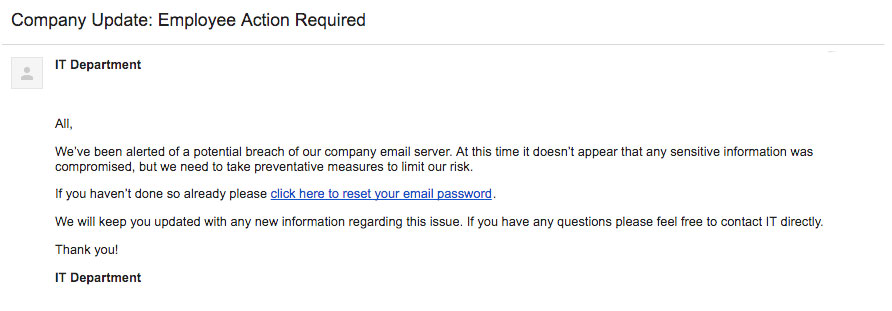
\includegraphics[scale=0.5]{msnr_phishing.jpg}
\end{center}
\caption{Primer pecanja }
\label{fig:phishing}
\end{figure}
% \end{primer}


\subsection{Drustvene mreze}
\label{subsec:podnaslovIP3}

Društvene mreže su jedna od najpopularnijih oblasti istraživanja i razvijanja. Ljudi zahvaljujuci njima menjaju način razmišljanja i drugačije imaju pogled na sve oko sebe. Neke od popularnijih mreža su Facebook, Skype, Twiter, Instagram, LinkedIn i skoro svi imaju nalog na bar jednoj mreži.Sve što korisnici postavljaju i šalju na društvenim mrežama predstavlja njihov prikaz ličnosti. Njihov cilj je međusobno druženje i komunikacija sa prijateljima, koje ne možemo svakodnevno da vidimo, ipak na njima ima dosta krađa indetiteta, napada na pojedince, svađa, pornografije i sličnih loših stvari. Dešava se da pojedini roditelji tek rođenoj deci otvaraju profile na nekoj od društvenih mreža, pa samim tim ih dovode u veliku opasnost postavljajući javno njihove slike,a da ne slute da te slike mogu biti zloupotrebljene. Na ovim mrežama se javalja veliki broj lažnih profila.
\begin{primer}
Napadači obično koriste te lažne profile sa velikom pažnjom, kako bi povećali nivo poverenja \cite{fakePr} . 
\end{primer}
Ukoliko dođe do napada na određeni pravi profil, dešava se da pored ukradenog indetiteta  napadači šire nepoželjan sadržaj, kao sto su eksplicitne fotografije i dokumenta. Oni koji prave profile sa tuđim indetitetom ili hakuju željene profile, obično veoma dobro poznaju tu osobu ,pa  mogu biti čak i članovi porodice. Svi ti lažni profili mogu biti veoma opasni ako se ne otkriju na vreme, pa oni predstavljaju sve veće probleme.

\subsection{Masovna kontrola, posmatranje i privatnost na Internetu}
\label{subsec:podnaslovIP4}

%?????????????
\indent\indent Prosečni korisnici Interneta uglavnom nisu ni svesni da za korišćenje najpopularnjih "besplatnih" Veb servisa (pretraživači, e-mail, društvene mreže..) za uzvrat odaju ogroman broj podataka i informacija o sebi. Zbog neinformisanosti imaju lažan osećaj sigurnosti i neosnovano poverenje da im je omogućena anonimnost. Većina tih servisa se, bez znanja korisnika, bavi masovnim skladištenjem podataka i njihovom analizom ((eng.~{\em data mining})). Rezultate dobijene iz analize podataka mogu koristiti za manipulaciju na raznim sektorima, poput ekonomskog tržista, političkih ciljeva, marketinga i slično. Pored obrade podataka društvenih masa, bez ikakvih ograničenja se mogu izdvojiti podaci i o pojedincima.
		
	Počinioci ovakvih radnji se uglavnom mogu svrstati u dve određene grupe, privatne korporacije i državne agencije. Motiv u slučaju privatnih korporacija je naravno profit. Dobro poznavanje tržista i korisnika njihovih proizvoda je ekvivalentno visokom profitu. Motiv kod državnih agencija je, naivno gledano, sigurnost države i njenih stanovnika (npr. sprečavanje terorizma). Iako je često dosta veći akcenat na kontroli i smanjenju privatnosti sopstvenih građana. Dalje ćemo kroz nekoliko najzanimljivijih primera koji su izloženi javnosti pokazati kako servise na Internetu treba koristiti sa dobrom dozom nepoverenja.\\
	
\textbf{Uzbunjivač (eng.~{\em whistleblower})} - \textit{naziv za hrabrog pojedinca koji iz moralnih razloga odlučuje da uz sopstveni rizik progovori o nezakonitim i neetičkim radnjama svojih nadređenih.}

\begin{primer}
	Edward Snowden, jedan od najpoznatijih uzbunjivača otkriva mnoge operacije državnih organizacija SAD koje narušavaju privatnost velikog dela korisnika Interneta. U dokumentima koje objavljuje pokazuje kolaboraciju mnogih država ("Five Eyes", alijansa koja se sastoji od Australije, Kanade, Novog Zelanda, Britanije i SAD-a) u projektima koji su korišćeni za globalno posmatranje i otkrivanje privatnih podataka na mreži.\cite{noPlaceToHide} Neki od značajnijih programa su koje je Edward izneo javnosti su:
\begin{itemize}
	\item \textbf{MUSCULAR}, presreće mnoštvo podataka pristupom kablovima ispod površine mora, kao i nelegalnim pristuom data centrima uglavnom korporacija Yahoo i Google. \cite{noPlaceToHide}
	\item \textbf{PRISM}, softver pod okriljem američke Nacionalne Sigurnosne Agencije (NSA). Program je pored velikih korporacija kao izvora privatnih podataka (Microsoft, Facebook, Google, Apple...) presretao i podatke u toku prenošenja na kičmenom stubu (engl.~{\em backbone}) Interneta. \cite{noPlaceToHide}
	\item \textbf{XKEYSCORE}, program za opšti pristup bilo kakvim informacijama koje prolaze kroz Internet. Jednostavnim upitom i pretragom pokazuje bilo čije e-mailove, privatne poruke, telefonske pozive, fajlove, lokacije i ostale razne informacije. Procena je da Xkeyscore dnevno prikupi oko 1.7 milijardu poruka, poziva i drugih podataka. \cite{noPlaceToHide}
	\item \textbf{BULLRUN}, služi za razbijanje enkriptovanih poruka na mreži. \cite{noPlaceToHide}
\end{itemize}
\end{primer}

\begin{primer}
	Makmilijan Šrems, tadašnji dvadeset trogodišnji student prava u
Austriji, je 2011-te godine od Facebook-a tražio sve privatne podatke koje su sakupili o njemu. Pored zahteva za podatke je i tužio Facebook jer su nelegalno prosleđivali privatne podatke korisnika društvene mreže projektu PRISM\cite{noPlaceToHide} za koji je zadužena NSA. Nakon dvogodišnje sudske parnice, Maks dobija od Facebook-a pdf fajl koji sadrži isključivo njegove lične podatke i koji ima čak 1200 stranica. \cite{marxSchremsFT}
\end{primer}

% https://www.pnas.org/content/111/24/8788
\begin{primer}
	Januara 2012-te, Facebook pravi psihološki eksperiment koji 
traje jednu nedelju. U eksperimentu učestvuje 689,003 profila koji su izloženi emotivnoj manipulaciji. Ovim se tragalo za odgovorom da li se emotivna zaraza može širiti kroz mrežu. Zapravo, Facebook je podelio učesnike testa na određene grupe, gde je svaka grupa dobijala isključivo objave koje izazivaju ili pozitivne ili negativne emocije na početnoj strani društvene mreže. To je rezultovalo u prenošenju emocija, gde je grupa koja je viđala samo pozitivne objave pokazala uvećane srećne emocije i analogno 	za grupu koja je izložena negativnim emocijama. \cite{facebookExperiment}
\begin{quotation}
	\textit{"We show, via a massive (N = 689,003) experiment on Facebook, that emotional states can be transferred to others via emotional contagion, leading people to experience the same emotions without their awareness.
"Data from a large real-world social network, collected over a 20-y period suggests that longer-lasting moods (e.g., depression, happiness) can be transferred through networks".}
\begin{flushright}
-\em{Deo zaključka iz originalnog naučnog rada.} \cite{facebookExperiment}
\end{flushright}
\end{quotation}
\end{primer}

\begin{primer}
	Sredinom 2009-te godine, Amazon izaziva veoma ironičnu 
situaciju. Nakon nekoliko hiljada prodatih e-book kopija knjige "1984" Džordža Orvela, ispostavlja se da izdavačka kuća tih kopija nema autorska prava. Amazon čitav problem rešava tako što bez znanja korisnika briše sve kopije na njihovim uređajima Kindle. Ovaj postupak je opisan kao "Orwellian" i potegao je mnoga pitanja o tome kolika prava Amazon ima. \cite{dataAndGoliath} \\
\textbf{"Orwellian"} - \textit{pridev koji opisuje nedostatak slobode i prava, propaganda, posmatranje, diktaturu...}\\
\end{primer}

\begin{primer}
	Jednostavna Android aplikacija "Brightest Flashlight 
Free" je pored svoje jedine funkcije, paljenja i gašenja blic LED svetla, nelegalno skupljala podatke u vidu lokacija korisnika. Aplikacija je imala izmedju 50 i 100 miliona korisnika i podaci o njihovim lokacijama su kupovale korporacije za marketing i reklame.\cite{dataAndGoliath}\cite{flashlightApp}\\
\end{primer}

\begin{primer}
	Mobilni telefoni su u stanju da svakog trenutka pokazuju lokaciju na kojoj se nalaze. Čak je i rađeno istraživanje gde su praćena kretanja određenog broja ispitanika preko moblinog telefona. Na osnovu skupljenih podataka o njihovim kretanjima, istraživači su uspeli sa iznenađujućom tačnošću da predvide njihove trase kretanja za naredna 24 sata. Za vreme revolucije u Kijevu, 2014-te, veliki broj učesnika protesta je dobilo SMS poruku upozorenja da učestvuju u demonstracijama. Poruku su dobile jedino osobe koje su bile u centru protesta, na osnovu lokacija koje je odašiljao njihov telefon. \cite{dataAndGoliath}
\end{primer}

	Vredni spomena su još neizbežnost skupljanja podataka od strane Googla uz pomoć njihovih {\em kolačići trećeg lica} (eng.~{\em third-party cookie}) i \textit{Google Analytics}. Google će dolaziti do vaših informacija čak i ako ne koristite njihov pretraživač. Oni mogu da skladište oko 15 eksabajta (1 eksabajt = $10^{18}$ bajtova). Procenjuje se da je Google najgori po pitanju skladištenju i korišćenju podataka korisnika. Poznata je i takozvana marketing diskriminacija. Funkcioniše tako što analizom podataka daje različite uslove i reklame korisnicima Interneta radi postizanja većeg profita. Kao primer, jedno od istraživanja pokazuje da su osobe ženskog pola više sklone kupovini kozmetičkih proizvoda ponedeljkom jer tim danom u nedelji imaju manji nivo samopouzdanja u odnosu na ostale dane. Naravno, stvari poput toga se koriste za postavljanje reklama u pravo vreme sve radi profita ne vodeći previše računa o etici ili moralnosti. \cite{dataAndGoliath} \cite{theNetDelusion}

	Ovo su samo od nekih mnogobrojnih primera koji nam pokazuju da korišćenje Interneta nije toliko "besplatno" i naivno koliko se misli. Iako se trenutno ne može uraditi mnogo stvari povodom toga, poželjno je što više proširiti informisanost o tome šta se sve zapravo dešava na mreži.

\section{Zavisnost od interneta}

\addcontentsline{toc}{section}{Literatura}
\appendix
\bibliography{seminarski} 
\bibliographystyle{plain}
\appendix
\end{document}
